\section{Method}
\label{sec:method}

We study \emph{ParT-EV}, a family of Particle Transformer extensions with
edge-conditioned value messages. We use \emph{EdgeValue} for the message
mechanism and \emph{ParT-EV} for models that include it. The main study retains
ParT's standard kinematic pair features and compares EdgeValue under shared
and layerwise attention bias.

\subsection{Particle attention and pair information}

Figure~\ref{fig:edgevalue-concept}(a) shows the two input streams of ParT-EV.
Particle features pass through an embedding with widths $(128,512,128)$
and eight particle self-attention blocks. In parallel, kinematic pair features
are embedded and supplied to every particle-attention block. The attention
width is $128$ with eight heads, giving head dimension $d_h=16$.
Following the Particle Transformer (ParT) backbone~\cite{Qu2022ParticleTransformer},
two class-attention blocks use the final particle representations to update
a learned class token. A linear classifier and the final softmax convert
this token into jet-class probabilities.
EdgeValue changes the particle-attention computation, leaving this class
readout unchanged. Our central question is whether using the existing pair
information to condition value messages improves ParT, and whether that
benefit depends on the choice of shared or layerwise attention bias.

\begin{figure}[!t]
 \centering
 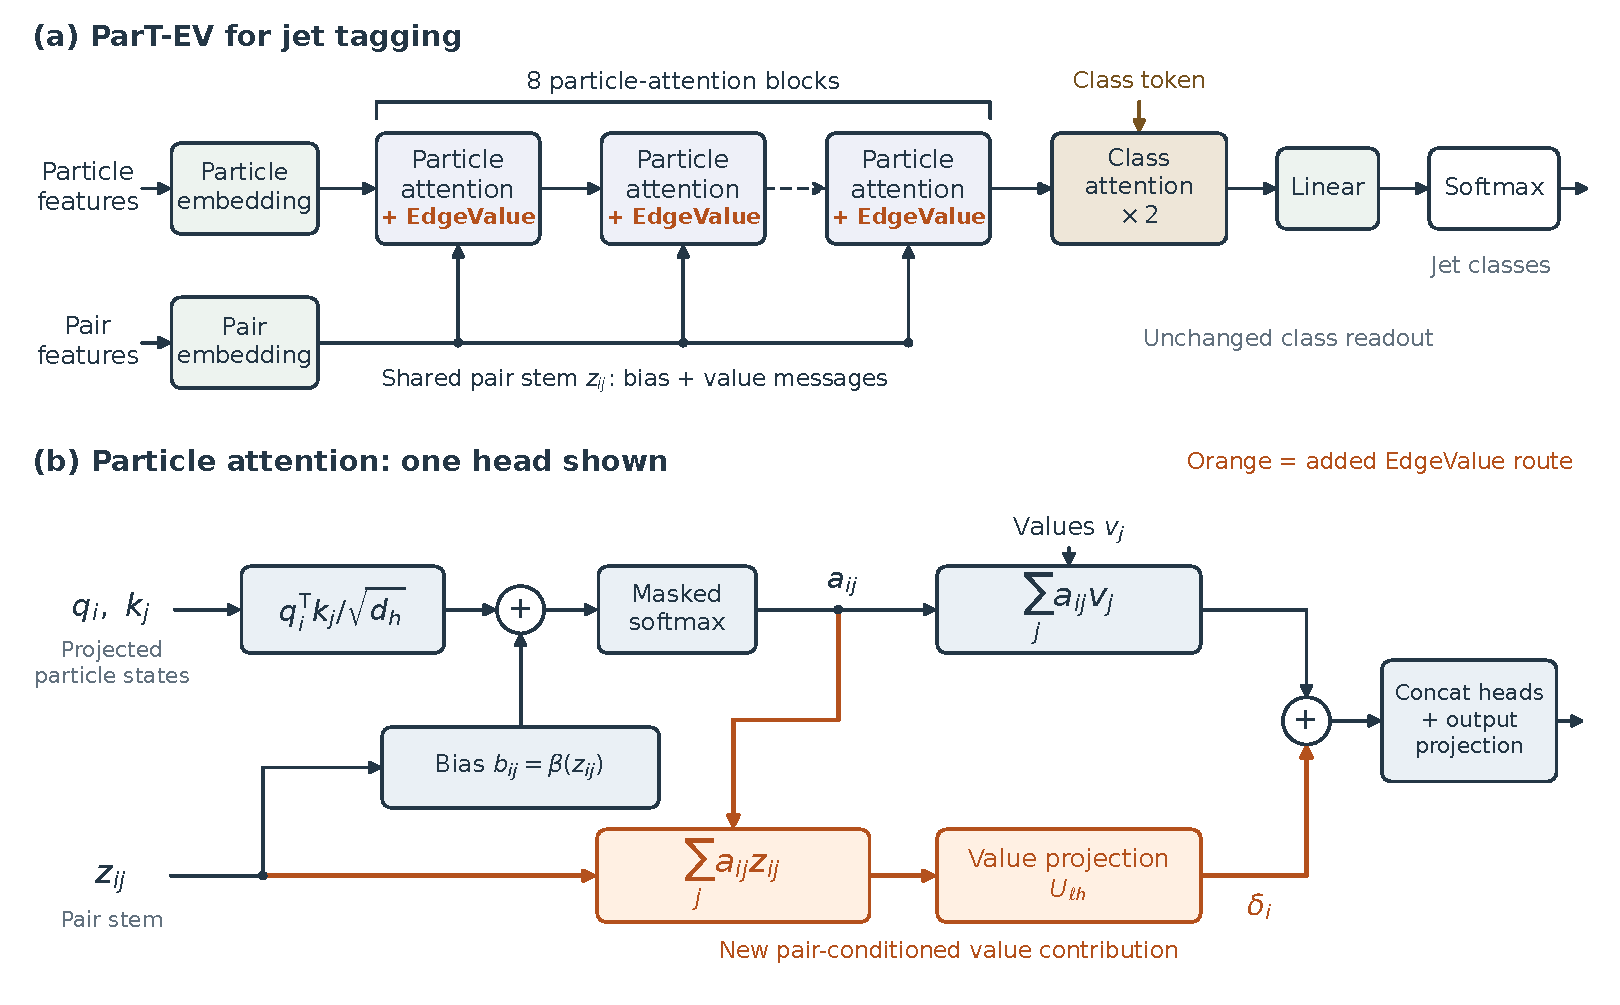
\includegraphics[width=\textwidth]{figures/edgevalue_architecture.pdf}
 \caption{ParT-EV architecture. (a) Particle and pair features follow parallel
 embedding streams; the pair stem is supplied to each of the eight
 particle-attention blocks. The class-attention readout and classifier retain
 the ParT design~\cite{Qu2022ParticleTransformer}. (b) One attention head:
 the usual pair-biased attention path is shown in dark blue. The added
 EdgeValue route (orange) aggregates pair embeddings with the same attention
 weights, projects the result with $U_{\ell h}$, and adds it to the ordinary
 value sum before head concatenation and output projection. Surrounding
 normalization, residual, and feed-forward operations are omitted.
 Evaluation-time weights are shown; layer/head indices are suppressed except
 on $U_{\ell h}$. The bias map may be shared or layerwise.}
 \label{fig:edgevalue-concept}
\end{figure}

For a valid query particle $i$ and context particle $j$, the baseline supplies four kinematic pair features,
\begin{equation}
 r_{ij}
 = \bigl(\Lambda(k_{t,ij}),\Lambda(\zeta_{ij}),
          \Lambda(\Delta_{ij}),\Lambda(m^2_{ij})\bigr),
 \label{eq:standard-pairs}
\end{equation}
where $\Lambda(x)=\log(\max\{x,10^{-8}\})$. Here $\Delta$ is separation in
rapidity--azimuth space, $k_t$ the relative transverse-momentum scale,
$\zeta$ the smaller transverse-momentum share, and $m^2$ the pair invariant
mass squared. The baseline therefore already incorporates pairwise kinematics
within global attention.

The upper path in Figure~\ref{fig:edgevalue-concept}(b) is the usual ParT
attention computation: a pair-derived bias is added to the query--key score
before a masked softmax determines the attention weights.

For layer $\ell$ and head $h$, biased attention is~\cite{Vaswani2017Attention,Qu2022ParticleTransformer}
\begin{equation}
 \begin{aligned}
 L^{\ell h}_{ij}
 &=\frac{(q_i^{\ell h})^{\mathsf T}k_j^{\ell h}}{\sqrt{d_h}}
       +b^{\ell h}_{ij},\\
 a^{\ell h}_{ij}
 &=\frac{\exp L^{\ell h}_{ij}}
        {\sum_{k\in\mathcal V}\exp L^{\ell h}_{ik}},
 \qquad i,j\in\mathcal V.
 \end{aligned}
 \label{eq:biased-attention}
\end{equation}
Here $\mathcal V$ is the set of valid constituents, so the normalization excludes
padded keys and permits self-attention ($j=i$). We write
$\widetilde a=\operatorname{Dropout}(a)$ for the attention weights after
training-time dropout; at evaluation $\widetilde a=a$.
Bias-only attention aggregates $\sum_{j\in\mathcal V}\widetilde a^{\ell h}_{ij}v_j^{\ell h}$:
relations affect the weights, while each context value remains independent of its query.

\subsection{Shared and layerwise interaction biases}

A three-stage, width-64 pair network maps the standard pair features to a
common relation stem $z_{ij}=\phi(r_{ij})\in\mathbb R^{64}$, corresponding
to the lower embedding stream in Figure~\ref{fig:edgevalue-concept}(a).
The bias branch in panel~(b) converts this representation into one scalar
bias per attention head.
Shared bias uses one head-output map $\beta$ in all particle layers,
$b^{\ell h}_{ij}=\beta_h(z_{ij})$. Layerwise bias uses independently trainable
maps $\beta_\ell$, so $b^{\ell h}_{ij}=\beta_{\ell h}(z_{ij})$, while retaining
the common stem. The layerwise maps, including their output normalization,
have identical initial parameters.

\subsection{Relation-conditioned value messages}
\label{sec:edgevalue}

Pairwise attention bias influences how strongly a query receives a context
particle's value. In bias-only ParT, however, the underlying value vector
$v_j^{\ell h}$ is the same for every query receiving information from $j$
within that layer and head. EdgeValue also makes the message content depend
on the relation between the two particles.

The orange route in Figure~\ref{fig:edgevalue-concept}(b) gives the pair
embedding a second role: in addition to supplying an attention bias, it
contributes a learned vector to the value message. The extra vector for
pair $(i,j)$ is $U_{\ell h}z_{ij}$, and it receives the same attention weight
as the ordinary value $v_j^{\ell h}$. Building on relation-aware value
messages~\cite{Shaw2018Relative}, ParT-EV therefore uses
\begin{align}
 y_i^{\ell h}
 &=\sum_{j\in\mathcal V}\widetilde a^{\ell h}_{ij}
   \left(v_j^{\ell h}+U_{\ell h}z_{ij}\right),
 \label{eq:edgevalue}\\
 \delta_i^{\ell h}
 &=\sum_{j\in\mathcal V}\widetilde a^{\ell h}_{ij}U_{\ell h}z_{ij},
 \qquad U_{\ell h}\in\mathbb R^{16\times64}.
 \label{eq:edgevalue-message}
\end{align}
Here $y_i^{\ell h}$ is the head aggregate before the existing output projection,
and $\delta_i^{\ell h}$ is the addition to the ordinary weighted value sum.
Both terms use the same attention weights $\widetilde a$ and the same
training-time attention-dropout realization.

The figure shows an equivalent, efficient ordering of this computation.
Because $U_{\ell h}$ is linear and independent of $i$ and $j$, the pair
embeddings can be aggregated before projection:
\begin{equation}
 \delta_i^{\ell h}
 =U_{\ell h}\left(\sum_{j\in\mathcal V}
   \widetilde a^{\ell h}_{ij}z_{ij}\right).
 \label{eq:edgevalue-efficient}
\end{equation}
The first orange block computes the attention-weighted sum of pair embeddings;
the second maps it from 64 channels to the 16-dimensional head value space.
At the addition node on the right, this contribution joins the ordinary
weighted value sum. Head outputs are then concatenated and passed through
the existing output projection. This ordering avoids materializing a separate
pair-value vector for every head, although pair features and attention weights
still require quadratic storage.

The pair stem is encoded from the input descriptors and shared across
particle-attention layers, rather than updated from their evolving particle
states. Its encoder is trained jointly with the classifier. Each layer and
head has its own projection $U_{\ell h}$, so the same pair representation
can contribute differently at different depths and through different heads.
The orange route is present under either bias scheme: EdgeValue requires
neither layerwise bias nor additional pair descriptors.

The value-message projections are bias-free. Within each layer, their stacked
$8\times16\times64$ parameter tensor is initialized with Xavier-uniform
initialization and optimized jointly with the rest of the network. Setting all
$U_{\ell h}=0$ removes the additional term and recovers the corresponding
bias-only attention operation for fixed remaining parameters. Invalid pair
stems and padded-query edge contributions are zeroed. The surrounding
normalization, residual, and feed-forward operations remain unchanged.
Applied to all eight particle-attention blocks in panel~(a), the projections
add $8\times8\times16\times64=65{,}536$ trainable parameters relative to
the matching bias-only path.
